% Template LaTeX document for CSSR4Africa Deliverables
% Adapted from documents prepared by EPFL for the RobotCub project
% and subsequently by the University of Skövde for the DREAM project
%
% DV 28/06/2023

\documentclass{CSSRforAfrica}

\usepackage[titletoc,title]{appendix}
\usepackage[colorlinks, urlcolor=blue, linkcolor=black, citecolor=black]{hyperref}
\usepackage{latexsym}
\usepackage{comment}
\usepackage{multirow}
\usepackage{subcaption}
\usepackage{tabularx}
\usepackage[breakable,skins,most]{tcolorbox} % Consolidated tcolorbox options
\usepackage{tabularx,colortbl}
\usepackage[tikz]{bclogo} % for boxes
\usepackage{ragged2e}
\usepackage{dirtree}
\usepackage{listings}
\usepackage{textcomp}
\usepackage{natbib}
\usepackage{url}
\usepackage{graphicx}
\usepackage{array}
\usepackage{longtable}
\usepackage{algorithm}
\usepackage{algorithmicx}
\usepackage{algpseudocode}
\usepackage{makecell}

%%% for listing %%%%%%%%%%%%%%%%%%%%%%%%%%%%%%
\captionsetup[figure]{format=hang}
\usepackage{xcolor}
\definecolor{codegreen}{rgb}{0,0.6,0}
\definecolor{codegray}{rgb}{0.5,0.5,0.5}
\definecolor{codepurple}{rgb}{0.58,0,0.82}
\definecolor{backcolour}{rgb}{0.95,0.95,0.92}
\definecolor{greenyellow}{rgb}{0.8, 0.7, 0.10} % Example values, adjust as needed

\lstdefinestyle{withoutNumbering}{
	backgroundcolor=\color{backcolour},   
	commentstyle=\color{codegreen},
	keywordstyle=\color{magenta},
	stringstyle=\color{codepurple},
	basicstyle=\ttfamily\small,
	breakatwhitespace=false,         
	breaklines=true,                 
	captionpos=b,                    
	keepspaces=true,                 
	showspaces=false,                
	showstringspaces=false,
	showtabs=false,                  
	tabsize=2
}
%%%%%%%%%%%%%%%%%%%%%%%%%%%%%%%%%%%%%%%%%%%%%%%%%%%
\definecolor{backcolour}{rgb}{0.95,0.95,0.95}
\definecolor{irongray}{HTML}{6D6E71}
\definecolor{LightGray}{gray}{0.9}

\newcommand{\blank}{~\\}
\newcommand{\checkbox}{{~~~~~~~\leavevmode \put(-7,-1.5){  \huge $\Box$  }}}

\begin{document}
\input{epsf}

%%
%% SHOULD NOT NEED TO BE CHANGED BEFORE THIS POINT
%% ------------------------------------------------
%%


\deliverable{D4.2.2}  
\title{D4.2.2 Face and Mutual Gaze Detection and Localization}  

\leadpartner{Carnegie Mellon University Africa} % REPLACE with partner name: Carnegie Mellon University Africa or The University of the Witwatersrand
\partner{}                                      

\revision{1.3} 
\deliverabledate{31/12/2023}  
\submissiondate{21/02/2025}  
\revisiondate{20/06/2025}   
\disseminationlevel{PU}
\responsible{Yohannes Haile}  


%%
%% Create the titlepage
%%

\maketitle
 

\section*{Executive Summary}
%===============================================================
\label{executive_summary}
%%\addcontentsline{toc}{section}{Executive Summary}
Deliverable D4.2.2 focuses on the development of a ROS node that detects and localizes human faces under various conditions and determines whether mutual gaze is established between the Pepper robot and the human user through head pose estimation. This deliverable includes the implementation of a ROS node called \texttt{faceDetection}, accompanied by a comprehensive report documenting the development process, refinement of requirements, and a detailed specification of the node's functional characteristics. Additionally, it provides a user manual with clear instructions on building and launching the ROS node. The design of the interface covers input, output, and control data, with suitable data structures and code that adhere to the software engineering standards established by the project. The functionality of the \texttt{faceDetection} node is thoroughly tested and validated using various test cases, including scenarios with different lighting conditions, occlusions, and varying distances between the robot and the user. The node is also tested on the Pepper robot to confirm its reliability and real-time performance, ensuring it meets the intended objectives effectively.

\newpage
 
 
\pagebreak
\tableofcontents
\newpage


\section{Introduction}
%===============================================================
This document outlines the development and implementation of a ROS node for face detection, localization, and mutual gaze detection using head pose estimation for the Pepper robot. The primary goal of this node is to enhance the interaction capabilities of the Pepper robot, allowing it to identify and track human faces within its environment, which serves as a cornerstone for creating natural and intuitive interactions. The mutual gaze detection functionality further strengthens this interaction by leveraging head pose estimation to identify moments when users establish eye contact with the robot—an essential component of engaging and socially aware behavior.

The deliverable includes a detailed report documenting the complete software development life cycle for the face detection and localization module. The requirements definition process is thoroughly covered, ensuring that all functional necessities are carefully aligned with the project's objectives. This section also highlights any identified misalignment or challenges that may arise during the development process and how they are addressed. The module design section provides an in-depth description of the face detection and mutual gaze localization functionality, covering critical aspects such as input, output, and control data.

The operation of the module is guided by parameters defined in a configuration file, which is structured as a list of key-value pairs in the \texttt{face\_detection\_configuration.json} file. This configuration allows for flexible and scalable customization of the module's behavior to suit various operating conditions and requirements. Furthermore, the document emphasizes the importance of robust design principles to ensure the module's reliability and performance in real-time applications.

\newpage

\section{Requirements Definition}
The face and mutual gaze detection and localization module is designed to meet the following requirements, ensuring seamless integration with the Pepper robot and its ROS-based ecosystem. The key requirements for the module are as follows:
\subsection*{Face Detection}
\begin{itemize}
	\item Detect human faces in the robot’s field of view using an RGB image as input.
	\item Detect and localize all faces in the field of view when multiple people are present.
	\item Localize faces by determining their position in the image and drawing bounding boxes.
	\item Identify the centroid coordinates of each bounding box.
	\item Determine the depth of all the faces detected.
\end{itemize}

\subsection*{Face Labeling and Consistency}
\begin{itemize}
	\item Assign unique labels to detected faces (e.g., ``Face 1").
	\item Maintain consistent labeling of the same face across consecutive image frames, provided the spatial displacement is within a defined tolerance.
	\item Reassign new labels to reappearing faces if not detected for a configurable number of images.
\end{itemize}

\subsection*{Gaze Direction Estimation}
\begin{itemize}
	\item Analyze head pose to estimate gaze direction, enabling the detection of mutual gaze between the robot and the user.
\end{itemize}

\subsection*{Configurable Parameters}
\begin{itemize}
	\item Allow customization through a configuration file (\texttt{face\_detection\_configuration.json})
\end{itemize}

\subsection*{Input/Output Specifications}
\begin{itemize}
	\item \textbf{Input}: RGB-D image from a robot camera or external camera.
	\item \textbf{Output}: Annotated images with bounding boxes and labeled face records published to the \texttt{/faceDetection/data} topic.
\end{itemize}

\subsection*{Verbose Mode}
\begin{itemize}
	\item Provide optional diagnostic output and visual debugging through an OpenCV window.
\end{itemize}


\subsection*{Misalignment of the module}
Due to the poor quality of the robot’s onboard camera, it was necessary to use an external camera. Hence, the depth information provided by the Pepper's camera is low quality hence the depth information (distance of the faces from the camera) isn't accurate. In addition, this module doesn't support the simulator. 

\newpage	

\section{Module Specifications}
The face detection module, implemented as a ROS node named faceDetection, is designed to detect faces within Pepper robot's field of view and determine their location and gaze direction in the image frame of reference. The module provides labeled, color-coded bounding boxes around each detected face and tracks these label across successive images for coherent detection. The module doesn't  perform face recognition but ensure consistency in labeling based on spatial proximity and configurable tolerance settings.

The inputs for this module are an RGB image from the robot's camera or external camera (Intel RealSense D435i), the depth iamge from the robot's depth sensors or an external RGB-D camera (Intel Realsense D435i).

The outputs for this module are annotated RGB image with bounding boxes around detected faces and an array of records is published with the following message \texttt{faceDetection/data} topic:
\begin{itemize}
	\item Face label representing as number
	\item 3D image coordinates of the bounding box centroid
	\item True/False value determining whether a mutual gaze is established.
	\item Width and Height of the bounding box.
	
\end{itemize}

The module utilizes two methods for face detection: \texttt{MediaPipe} and a \texttt{YOLO} (You Only Look Once) \cite{yolo} based face detection model. Each method is optimized for different scenarios, giving the flexibility to the user to select between these two algorithms based on their specific requirements.

\texttt{MediaPipe} is ideal for face detection within shorter distances and when processing is limited to CPU-based computing. It efficiently detects facial landmarks, including key points such as the distance between the eyes, nose, and mouth, which are essential for inferring the 3D orientation of the head pose. However, its performance and detection range are limited when faces are located farther from the camera.

On the other hand, the \texttt{YOLO-based model} is a deep learning approach designed to detect human heads at greater distances, leveraging GPU acceleration for robust and accurate face detection, even in challenging environments. Once a face is detected, the model applies \texttt{SixDRep (6D Rotation Representation for Unconstrained Head Pose Estimation)} \cite{sixdrepnet} to determine the head’s orientation. This method offers a representation of the head’s rotation across six degrees of freedom, allowing the system to accurately assess mutual gaze.

By providing the option to choose between MediaPipe and YOLO, the module ensures flexibility across various settings. MediaPipe can be selected for lightweight, close-range scenarios, while YOLO can be chosen for long-range detection and environments where GPU resources are available.

If verbosemode is set to True in the configuration file, an OpenCV window displays the detected face's bounding box and indicate whether mutual gaze is established. Each detected face is assigned a unique label. This provides real-time visualization and tracking for face detection and gaze estimation. 

A unit test is developed to cover various scenarios, including multiple faces, partial occlusion, variable lighting conditions, and label reassignment when faces disappear. The tests is conducted using a driver-stub test platform, which utilizes recorded color and depth images stored in the data folder. Additionally, the unit tests can be executed directly on the physical robot to validate real-world performance.

\newpage
\section{Module Design}
\subsection*{Image Input}
The primary input for the ROS node is the Intel RealSense camera mounted on top of Pepper's head. As an alternative, the Pepper camera can also be used by configuring the camera parameter in the configuration file. However, as noted in section 2 the depth camera has very low quality. The Intel RealSense camera provides both RGB and depth images at various resolutions and frame rates, which can be customized through the launch file parameters. Table \ref{table: Intel RealSense D435i stream configuration} below outlines the available resolution and frame rate configurations for the Intel RealSense camera.

\begin{table}[h!]
	\centering
	\begin{tabular}{|>{\centering\arraybackslash}m{2.5cm}|>{\centering\arraybackslash}m{3cm}|>{\centering\arraybackslash}m{3.0cm}|>{\centering\arraybackslash}m{5cm}|}
		\hline
		\rowcolor{blue!20} % Light blue background color
		\textbf{Format} & \textbf{Resolution} & \textbf{Frame Rate (FPS)} & \textbf{Comment} \\ \hline
		\multirow{6}{*}{Z [16 bits]} & 1280x720 & 6, 15, 30 & \multirow{6}{*}{Depth} \\ \cline{2-3}
		& 848x480 & 6, 15, 30, 60, 90 & \\ \cline{2-3}
		& 640x480 & 6, 15, 30, 60, 90 & \\ \cline{2-3}
		& 640x360 & 6, 15, 30, 60, 90 & \\ \cline{2-3}
		& 480x270 & 6, 15, 30, 60, 90 & \\ \cline{2-3}
		& 424x240 & 6, 15, 30, 60, 90 & \\ \hline
		
		\multirow{9}{*}{YUY2 [16 bits]} & 1920x1080 & 6, 15, 30 & \multirow{9}{*}{\parbox{5cm}{Color Stream from RGB camera \\ (Camera D415 \& D435/D435i)}} \\ \cline{2-3}
		& 1280x720 & 6, 15, 30 & \\ \cline{2-3}
		& 960x540 & 6, 15, 30, 60 & \\ \cline{2-3}
		& 848x480 & 6, 15, 30, 60 & \\ \cline{2-3}
		& 640x480 & 6, 15, 30, 60 & \\ \cline{2-3}
		& 640x360 & 6, 15, 30, 60 & \\ \cline{2-3}
		& 424x240 & 6, 15, 30, 60 & \\ \cline{2-3}
		& 320x240 & 6, 30, 60 & \\ \cline{2-3}
		& 320x180 & 6, 30, 60 & \\ \hline
	\end{tabular}
	\caption{Stream Configurations for Depth and Color for Intel RealSense D435i. See the official datasheet: \href{https://cdrdv2-public.intel.com/841984/Intel-RealSense-D400-Series-Datasheet.pdf}{Intel RealSense D400 Series Datasheet}.}
	\label{table: Intel RealSense D435i stream configuration}
\end{table}

\subsection*{Algorithms}
\subsubsection*{MediaPipe}
MediaPipe is open-source framework developed by Google that provides efficient solution for real-time computer vision application. Among the various capablitlies, MediaPipe can be utilized for head pose estimation by leveraging its face detection and face landmark modules. The process involves detecting key facial landmarks, such as the eyes, nose and mouth, to determine the orientation of the head in 3D space. MediaPipe's Face Mesh module identifies 468 distinct facial landmarks with high precision, allowing for robust tracking of head movements. Once these landmarks are detected, they are used as input to compute the head's rotation and translation relative to the camera coordinate system. Figure \ref{fig: MediaPipe Face land marks} shows the landmarks detected on the human face. 

\newpage

\begin{figure}[!hbpt]
	\centering
	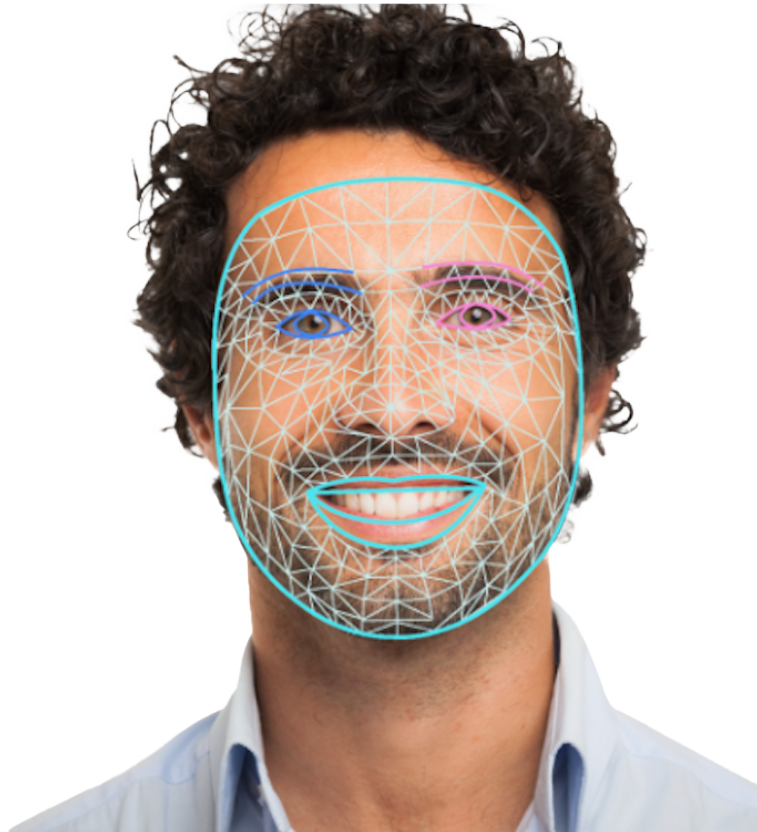
\includegraphics[scale=0.3]{images/MediaPipe_FaceLand_Marks.png}
	\caption{MediaPipe Face land marks \cite{mediapipe_face_landmarker}.}
	\label{fig: MediaPipe Face land marks}
\end{figure}

By fitting a 3D face model to the detected 2D landmarks using Perspective-n-Point(PnP), it calculates Euler angles (yaw, pitch, and roll) to represent the head’s orientation. 

\subsubsection*{SixDRepNet}
SixDRepNet is a deep learning-based model designed specifically for head pose estimation. Unlike traditional methods like MediaPipe, which rely on 2D-to-3D correspondences and facial landmarks, SixDRepNet takes a direct regression approach. It predicts the yaw, pitch, and roll angles directly from input images, without requiring explicit 3D landmark annotations or predefined face models. The process begins with YOLO, which detects the face in the input image and generates a bounding box. The detected face region is then cropped and resized to the required input dimensions of 224 × 224 pixels for the head pose estimation model. The preprocessed face image is fed into SixDRepNet, which outputs a 6D rotation representation. This representation is converted to a rotation matrix and used to compute the head’s yaw, pitch, and roll angles.

\subsubsection*{Centroid Tracker}
For tracking faces across frames, the centroid tracker is used together with MediaPipe. The tracker ensures the detected faces remains consistently tracked even as they move or momentrily disappear. Mediapipe detects facial landmarks and provides the bounding boxes around faace in each frame, while the centroid Tracker assigns and maintains unique IDs for each detected face. It calculates the centroid of the bounding boxes and tracks it across consecutive frames by measuring the Euclidean distance to match centroids. If a match is found, the corresponding face ID is updated; otherwise, a new ID is assigned. The tracker handles cases where faces temporarily disappear by keeping track of missed detection and deregistering them only after a set threshold of consecutive frames.

\newpage

\begin{algorithm}
	\caption{Centroid Tracker Algorithm}
	\textbf{Require:} Detected centroids $C_t$ at time $t$, tracked objects $O_{t-1}$ from time $t-1$ \\
	\textbf{Ensure:} Updated object IDs and centroids $O_t$
	\begin{algorithmic}[1]
		\If{$O_{t-1}$ is empty}
		\ForAll{centroid $c \in C_t$}
		\State \textbf{Register} $c$ as a new object with unique ID
		\EndFor
		\Else
		\State Compute distance matrix $D$ between $C_t$ and $O_{t-1}$
		\State Match centroids using nearest-neighbor approach
		\ForAll{matched pair $(o, c)$}
		\State Update object $o$ with new centroid $c$
		\State Reset disappearance counter for $o$
		\EndFor
		
		\ForAll{unmatched objects in $O_{t-1}$}
		\State Increment disappearance counter
		\If{counter exceeds threshold}
		\State \textbf{Deregister} the object
		\EndIf
		\EndFor
		
		\ForAll{unmatched centroids in $C_t$}
		\State \textbf{Register} centroid $c$ as a new object with unique ID
		\EndFor
		\EndIf
		\State \Return updated objects $O_t$
	\end{algorithmic}
\end{algorithm}

\subsubsection*{SORT (Simple Online and Realtime Tracker)}
The SORT algorithm is a lightweight multi-object tracking method that combines Kalman filtering for motion prediction and the Hungarian algorithm for data association. The process begins with detecting a face using an Intel RealSense camera mounted on Pepper's head. YOLO is employed for head detection, after which the Kalman filter predicts the motion of detected objects in subsequent frames. To associate new detections with existing tracks, SORT utilizes the Hungarian algorithm with Intersection over Union (IoU) as the matching criterion. Once matches are found, the Kalman filter updates its state with the latest information. Tracks that do not find a match are marked as lost and eventually deleted, while new detections initiate new tracks \cite{SORT}.

\newpage

\begin{algorithm}
	\caption{SORT Algorithm}
	\textbf{Require:} Detected bounding boxes $B_t$ at time $t$, tracked objects $O_{t-1}$ from time $t-1$ \\
	\textbf{Ensure:} Updated object IDs and bounding boxes $O_t$
	\begin{algorithmic}[1]
		\If{$O_{t-1}$ is empty}
		\ForAll{bounding box $b \in B_t$}
		\State \textbf{Register} $b$ as a new object with a unique ID
		\EndFor
		\Else
		\State Predict new positions of tracked objects using the \textbf{Kalman filter}
		\State Compute the cost matrix $D$ using \textbf{Intersection over Union (IoU)} between $B_t$ and predicted objects
		\State Solve the assignment problem using the \textbf{Hungarian algorithm}
		
		\ForAll{matched pairs $(o, b)$}
		\State Update object $o$ with new bounding box $b$
		\State Reset disappearance counter for $o$
		\EndFor
		
		\ForAll{unmatched objects in $O_{t-1}$}
		\State Increment disappearance counter
		\If{counter exceeds threshold}
		\State \textbf{Deregister} the object
		\EndIf
		\EndFor
		
		\ForAll{unmatched bounding boxes in $B_t$}
		\State \textbf{Register} bounding box $b$ as a new object with a unique ID
		\EndFor
		\EndIf
		\State \Return updated objects $O_t$
	\end{algorithmic}
\end{algorithm}
\vspace{-0.3cm}

Figure \ref{fig: SORT Diagrams} illustrates the complete process of SORT tracking.

\begin{figure}[!hbpt]
	\centering
	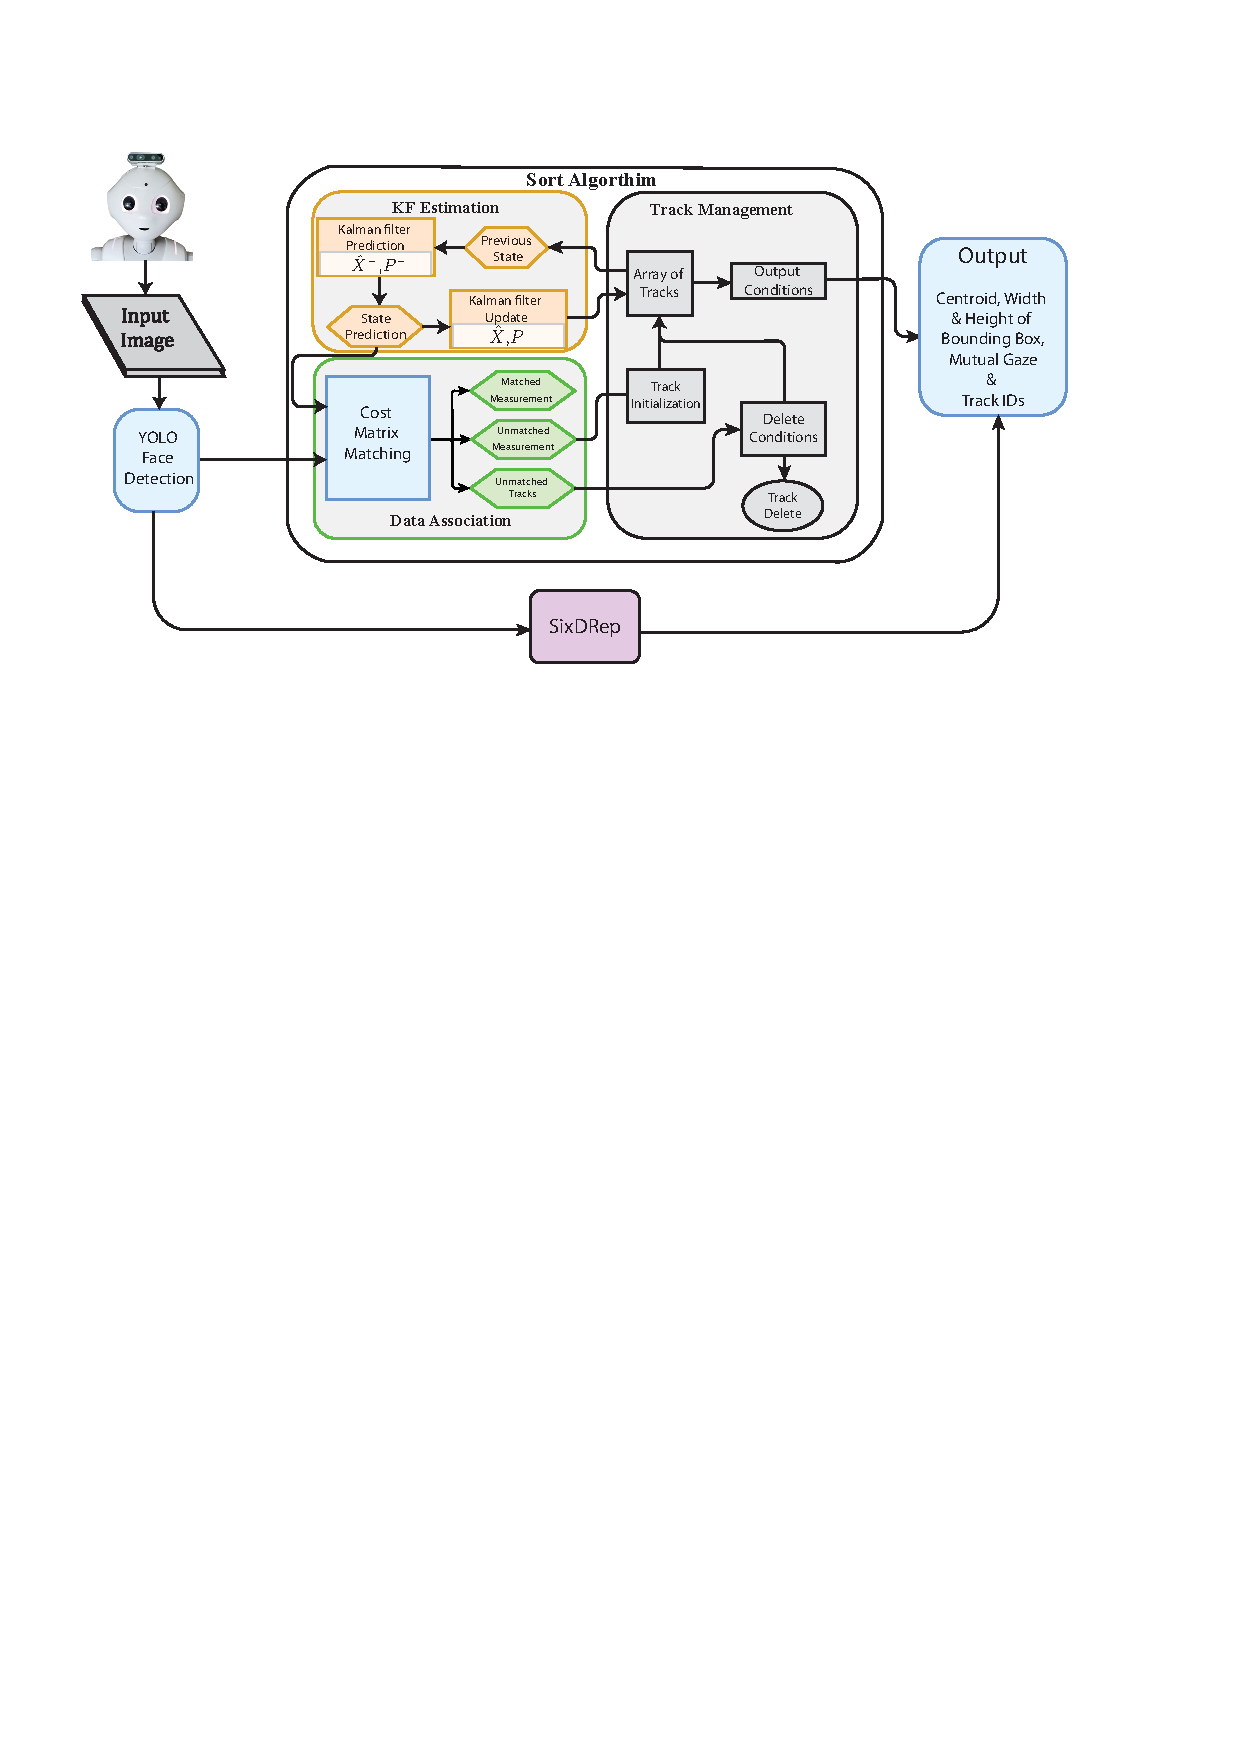
\includegraphics[scale=0.8]{images/SORT_Diagram.pdf}
	\caption{SORT Diagram.}
	\label{fig: SORT Diagram}
\end{figure}

\newpage

\section{Implementation}
\subsection*{File Organization}
The source code for conducting face detection, mutual gaze detection, and localization is structured into three primary components: {\fontsize{9.0}{10.0}\selectfont\texttt{{face\_detection\_application}, \texttt{face\_detection\_implementation}}, and \small{\texttt{face\_detection\_tracking}}. The \texttt{face\_detection\_implementation} component encapsulates all the essential functionality required for executing both face detection and mutual gaze detection, utilizing \texttt{MediaPipe} and \texttt{SixDRepNet}. The \texttt{face\_detection\_tracking} component, on the other hand, manages tracking functionality by employing either the Centroid Tracker or \texttt{SORT} (Simple Online and Realtime Tracking). Additionally, the face detection system is equipped with the capability to process various files critical for testing, such as configuration files, input files, and topic files. Meanwhile, the {\fontsize{8.0}{9.0}\selectfont{\texttt{face\_detection\_application}}} component serves as the entry point, invoking the main functions to run the face detection node and executing the functions defined within \texttt{face\_detection\_implementation}.\\

Figure \ref{fig:face_detection_directory} shows the file structure of the face detection package.

\begin{figure}[h]	
	\renewcommand*\DTstyle{\ttfamily}
	\dirtree{%
		.1 cssr\_system.
		.2 face\_detection.
		.3 config.
		.4 face\_detection\_configuration.json.
		.3 data.
		.4 pepper\_topics.dat.
		.3 launch.
		.4 face\_detection\_launch\_robot.launch.
		.3 models.
		.4 face\_detection\_goldYOLO.onnx.
		.4 face\_detection\_sixdrepnet360.onnx.
		.3 msg.
		.4 face\_detection\_msg\_file.msg.
		.3 src.
		.4 face\_detection\_application.py.
		.4 face\_detection\_implementation.py.
		.4 face\_detection\_tracking.py.
		.3 face\_detection\_requirements\_x86.txt.
		.3 README.md.
		.2 CSSR4AfricaLogo.svg.
		.2 CMakeLists.txt.
		.2 Package.xml.
	}
	\caption{File structure of the face detection system.}
	\label{fig:face_detection_directory}
\end{figure}

\newpage
\subsection*{UML Diagram for the Face and Mutual Gaze Detection and Localization Module}
The UML diagram provides a clear structural representation of the Face and Mutual Gaze Detection and Localization Module, illustrating the relationships between its core components. It highlights inheritance, where FaceDetectionNode serves as the base class, extended by MediaPipe and SixDRepNet for specialized face detection and head pose estimation. Associations between tracking components such as Sort, CentroidTracker, and TrackerUtils emphasize how detected faces are tracked using Kalman filtering and centroid-based methods. Composition relationships are depicted, showing that SixDRepNet integrates YOLOONNX for face detection as an essential part of head pose estimation, ensuring a modular and scalable system.\\

Figure \ref{fig: Face_implementation_UML} shows the UML diagram of face\_detection\_implementation.py.

\begin{figure}[!hbpt]
	\centering
	\hspace*{-0.5cm} % adjust the value as needed
	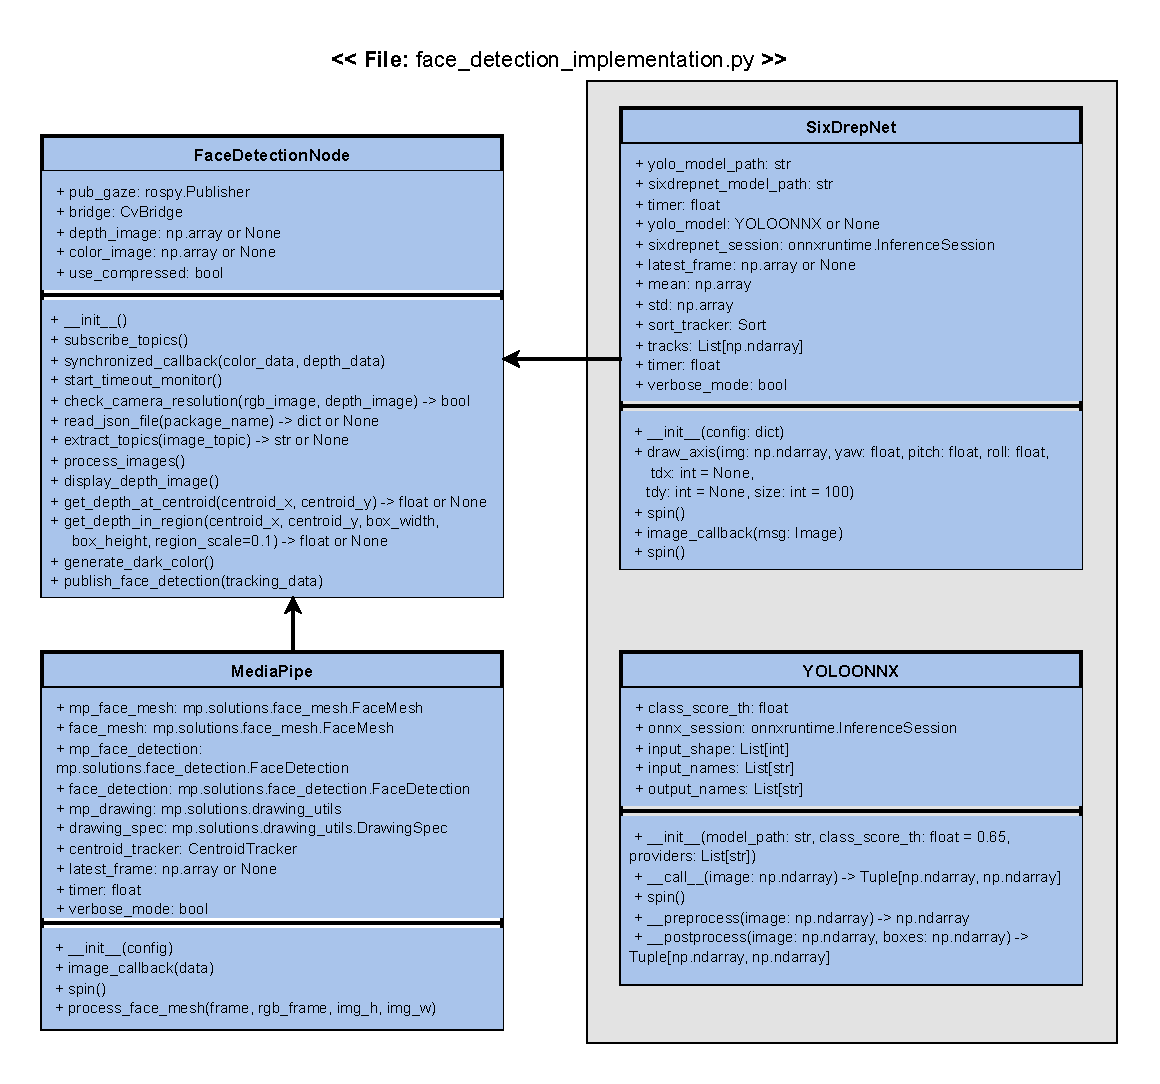
\includegraphics[scale=0.85]{images/Face_implementation_UML.pdf}
	\caption{Face detection implementation UML.}
	\label{fig: Face_implementation_UML}
\end{figure}

\newpage

Figure \ref{fig: Face detection tracking UML} shows the UML diagram of face\_detection\_tracking.py.

\begin{figure}[!hbpt]
	\centering
	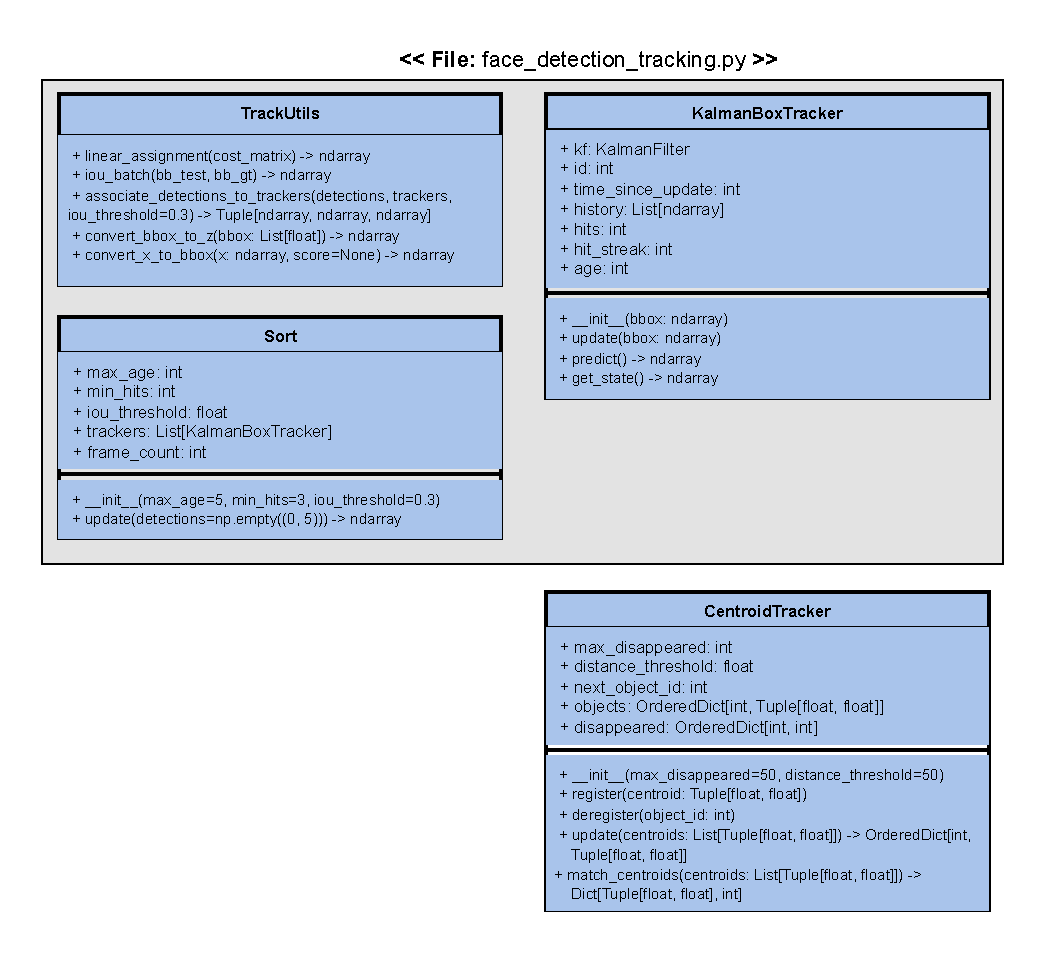
\includegraphics[scale=0.90]{images/Face_Tracking_UML.pdf}
	\caption{Face detection tracking UML.}
	\label{fig: Face detection tracking UML}
\end{figure}

\newpage

\subsection*{Configuration File}
The operation of the face detection node is determined by the contents of the configuration file that contains a list of key-value pairs as shown on the Table \ref{Table: configuration file for face detection node}.
The configuration file is named  \\
\texttt{face\_detection\_configuration.json}. 

\begin{table}[h!]
	\centering
	\begin{tabularx}{\linewidth}{| l | l | X|}
		\hline
		\rowcolor{blue!20} % Light blue background color
		\textbf{Key} & \textbf{Value} & \textbf{Description} \\
		\hline
		{\footnotesize \texttt{algorithm}}             & {\footnotesize \texttt{mediapipe or sixdrep}}   & {\small Specifies which algorithm to use.} \\
		\hline
		{\footnotesize \texttt{useCompressed}}          & {\footnotesize \texttt{true or false}}         & {\small Specifies to use compressed image or raw images.} \\
		\hline
		{\footnotesize \texttt{mpFacedetConfidence}}    & {\footnotesize \texttt{<number>}}              & {\small Specifies the confidence threshold for the MediaPipe face detection algorithm.} \\
		\hline
		{\footnotesize \texttt{mpHeadposeAngle}}        & {\footnotesize \texttt{<number>}}              & {\small Specifies the maximum angular deviation (in degrees) for MediaPipe head pose estimation.} \\
		\hline
		{\footnotesize \texttt{centroidMaxDistance}}    & {\footnotesize \texttt{<number>}}              & {\small Specifies the maximum allowed distance (in pixels) between centroids for tracking continuity.} \\
		\hline
		{\footnotesize \texttt{centroidMaxDisappeared}} & {\footnotesize \texttt{<number>}}              & {\small Specifies the maximum number of frames a centroid can disappear before being considered lost.} \\
		\hline
		{\footnotesize \texttt{sixdrepnetConfidence}}   & {\footnotesize \texttt{<number>}}              & {\small Specifies the confidence threshold for the SixDRepNet pose estimation algorithm.} \\
		\hline
		{\footnotesize \texttt{sixdrepnetHeadposeAngle}}& {\footnotesize \texttt{<number>}}              & {\small Specifies the maximum angular deviation (in degrees) for SixDRepNet head pose estimation.} \\
		\hline
		{\footnotesize \texttt{sortMaxDisappeared}}     & {\footnotesize \texttt{<number>}}              & {\small Specifies the maximum number of frames an object can disappear for SORT tracker before being removed.} \\
		\hline
		{\footnotesize \texttt{sortMinHits}}            & {\footnotesize \texttt{<number>}}              & {\small Specifies the minimum number of consecutive hits required for SORT tracker initialization.} \\
		\hline
		{\footnotesize \texttt{sortIouThreshold}}       & {\footnotesize \texttt{<number>}}              & {\small Specifies the Intersection over Union (IoU) threshold for SORT tracker associations.} \\
		\hline
		{\footnotesize \texttt{imageTimeout}}           & {\footnotesize \texttt{<number>}}              & {\small Timeout (seconds) for shutting down the node after video ends} \\
		\hline
		{\footnotesize \texttt{verboseMode}}           & {\footnotesize \texttt{true or false}}         & {\small Specifies whether diagnostic data is to be printed to the terminal and diagnostic images are to be displayed in OpenCV windows.} \\
		\hline
	\end{tabularx}
	\caption{Configuration file key-value pairs for the face detection node.}
	\label{Table: configuration file for face detection node}
\end{table}


\subsection*{Input File}
There is no input file the face detection node.

\subsection*{Output File}
There is no output file the face detection node. The node uses OpenCV to display the detected faces with bounding boxes and labels, and the mutual gaze detection.

\subsection*{Launch File}
The launch file \texttt{face\_detection\_launch\_robot.launch} is designed to initialize either Pepper's front camera or the Intel RealSense camera based on the specified configuration. It declares several parameters that can be customized to match your network settings and camera choice:
\begin{itemize}
	\setlength\itemsep{0em}
	\item \texttt{pepper\_robot\_ip}: specifies the IP address of the Pepper robot (default: \texttt{172.29.111.230}).
	\item \texttt{pepper\_robot\_port}: specifies the communication port for Pepper (default: \texttt{9559}).
	\item \texttt{network\_interface}: specifies the network interface name (default: \texttt{wlp0s20f3}).
	\item \texttt{roscore\_ip}: IP address of the ROS master (default: \texttt{127.0.0.1})
	\item \texttt{namespace}: sets the ROS namespace for the naoqi driver (default: \texttt{naoqi\_driver}).
	\item \texttt{camera}: selects the camera source; set to \texttt{pepper} for Pepper's front camera or \texttt{realsense} for the Intel RealSense camera (default: \texttt{realsense}).
\end{itemize}

The file sets the parameter \texttt{/faceDetection/camera} to the chosen camera and conditionally launches the corresponding nodes. If the \texttt{camera} parameter is set to \texttt{pepper}, the launch file starts the \texttt{naoqi\_driver} node using the provided IP, port, network interface, and namespace. Conversely, if \texttt{camera} is set to \texttt{realsense}, it includes the RealSense camera launch file with specified parameters for image resolution, frame rate, and depth alignment. Users can adjust these default values to suit their specific hardware configurations.

\subsection*{Models}
The face detection node uses two models for face detection and head pose estimation. The models are stored in the \texttt{models} directory. The models are shown in Table \ref{Table: Models for face detection node}.
\begin{table}[h!]
	\centering
	\begin{tabularx}{\linewidth}{| l | X |}
		\hline
		\rowcolor{blue!20} % Light blue background color
		\textbf{Models} & \textbf{Description} \\
		\hline
		{\footnotesize \texttt{face\_detection\_goldYOLO.onnx} }  & {\footnotesize YOLO-based face detection model.} \\
		\hline
		{\footnotesize \texttt{face\_detection\_sixdrepnet360.onnx} }  & {\footnotesize SixDRepNet head pose estimation model.} \\
		\hline
	\end{tabularx}
	\caption{Models used by the face detection node.}
	\label{Table: Models for face detection node}
\end{table}

\subsection*{Topics File} 
For the test, a selected list of the topics for the robot is stored in the topics file. The topic files are 
written in the .dat file format. The data file is written in key-value pairs where the key is the camera 
and the value is the topic. The topics file for the robot is named \texttt{pepper\_topics.dat}.

\newpage
\subsection*{Topics Subscribed}
The face detection node subscribes to the topics shown in Table \ref{Table: topic subscribed}.

\begin{table}[!h]
	\centering
	{\fontsize{7.0}{9.0}\selectfont % <- apply inside the table
		\begin{tabularx}{\linewidth}{| l | l | X |}
			\hline
			\rowcolor{blue!20}
			\textbf{Camera} & \textbf{Topic Name} & \textbf{Message Type} \\
			\hline
			\texttt{RealSenseCameraRGB} & \texttt{/camera/color/image\_raw} & \texttt{sensor\_msgs/Image} \\
			\hline
			\makecell[l]{\texttt{RealSenseCameraRGB} \\ (Compressed)} & \texttt{/camera/color/image\_raw/compressed} & \texttt{sensor\_msgs/CompressedImage} \\
			\hline
			\texttt{RealSenseCameraDepth} & \texttt{/camera/aligned\_depth\_to\_color/image\_raw} & \texttt{sensor\_msgs/Image} \\
			\hline
			\makecell[l]{\texttt{RealSenseCameraDepth} \\ (Compressed)} & \texttt{/camera/aligned\_depth\_to\_color/image\_raw/compressed} & \texttt{sensor\_msgs/CompressedImage} \\
			\hline
			\texttt{PepperFrontCamera} & \texttt{/naoqi\_driver/camera/front/image\_raw} & \texttt{sensor\_msgs/Image} \\
			\hline
			\texttt{PepperDepthCamera} & \texttt{/naoqi\_driver/camera/depth/image\_raw} & \texttt{sensor\_msgs/Image} \\
			\hline
		\end{tabularx}
	}
	\caption{Topics subscribed by the face detection node.}
	\label{Table: topic subscribed}
\end{table}

\subsection*{Topics Published}
The face detection node publishes to the topics shown in Table \ref{Table: topics published}.

\begin{table}[!h]
	\centering
	{\fontsize{8.5}{9.5}\selectfont
		\begin{tabularx}{\linewidth}{| l | l | X |}
			\hline
			\rowcolor{blue!20} % Light blue background color
			\textbf{Topic Name} & \textbf{Message Type} & \textbf{Description} \\
			\hline
			\texttt{/faceDetection/data}  & \texttt{faceDetection/face\_detection\_msg\_file} & \texttt{An array of records containing face labels, 3D image coordinates of the bounding box, width and height of the bounding box, and a boolean value indicating mutual gaze detection}. \\
			\hline
		\end{tabularx}
	}
	\caption{Topics published by the face detection node.}
	\label{Table: topics published}
\end{table}


\newpage
\section{Running the Face Detection Node}
To run the face detection node, the user must first install the necessary software packages as outlined in 
\href{https://cssr4africa.github.io/deliverables/CSSR4Africa_Deliverable_D3.3.pdf}{Deliverable 3.3}. The required packages
are listed in the \texttt{face\_detection\_requirements\_x86.txt} file. The user can follow the README file in the face detection
package to install the required packages. Refering to the implementation section of this deliverble report, the user must 
set the configuration file to the desired parameters. Using the key-value pair, the user can set the camera, algorithm, 
confidence threshold, and other parameters. The user can then run the face detection node by executing the following 
command in the terminal:

\begin{lstlisting}[style=withoutNumbering, language=bash]
# Launch either Pepper Camera or RealSense Camera from the launch file 
$ roslaunch cssr_system face_detection_launch_robot.launch camera:=pepper
# or
$ roslaunch cssr_system face_detection_launch_robot.launch camera:=realsense
\end{lstlisting}

Source the python environment you setup for face\_detection. 
\begin{lstlisting}[style=withoutNumbering, language=bash]
# Activate the virtual environment:
$ source $HOME/workspace/pepper_rob_ws/face_person_detection/bin/activate
\end{lstlisting}

\begin{lstlisting}[style=withoutNumbering, language=bash]
# Run the face detection node
$ rosrun cssr_system face_detection_application.py
\end{lstlisting}


If the user has set the verbose mode to True in the configuration file, the face detection node displays the detected 
faces with bounding boxes and labels, as well as the mutual gaze detection in an OpenCV window. The user can then interact 
	with the Pepper robot to establish mutual gaze and observe the system's response.

\newpage

\section{Unit Test}
The unit test is designed to validate the face detection node's functionality under various scenarios, including multiple faces, occlusions, and varying lighting conditions. 
The test can be performed using a driver-stub test platform, which utilizes recorded color and depth images stored in the data folder as a rosbag file. The unit test can also 
be executed directly on the physical robot to validate real-world performance. 

The face detection unit test file structure is as follows: 

\begin{figure}[h]	
	\renewcommand*\DTstyle{\ttfamily}
	\dirtree{%
		.1 unit\_test.
		.2 face\_detection\_test.
		.3 config.
		.4 face\_detection\_test\_configuration.json.
		.3 data.
		.4 face\_detection\_test\_input\_single\_face.bag.
		.4 face\_detection\_test\_input\_multiple\_faces.bag.
		.4 face\_detection\_test\_input\_mutual\_gaze.bag.
		.4 face\_detection\_test\_input\_lighting\_1.bag.
		.4 face\_detection\_test\_input\_lighting\_2.bag.
		.3 launch.
		.4 face\_detection\_test\_launch\_robot.launch.
		.4 face\_detection\_test\_launch\_test\_harness.launch.
		.3 msg.
		.4 face\_detection\_test\_msg\_file.msg.
		.3 src.
		.4 face\_detection\_test\_application.py.
		.4 face\_detection\_test\_implementation.py.
		.3 README.md.
		.2 CSSR4AfricaLogo.svg.
		.2 CMakeLists.txt.
		.2 Package.xml.
	}
	\caption{File structure of the face detection unit test.}
	\label{fig:face_detection_unit_test}
\end{figure}

The test cases for the face detection node that are going to be evaluated as shown in Table \ref{Table:face_detection_tests}.

\begin{longtable}{| l | p{10.5cm} |}
    \hline
    \rowcolor{blue!20} % Light blue background color
    \textbf{Test Case} & \textbf{Description} \\
    \hline
    \endfirsthead

    % Continuation header for the next pages
    \hline
    \rowcolor{blue!20} 
    \textbf{Test Case} & \textbf{Description} \\
    \hline
    \endhead

    % Table content
    \text{Single Face Detection} & Verify the face detection node's ability to detect and localize a single face in the image frame, as well as evaluate the distance at which the face is detected. \\
    \hline
    \text{Multiple Face Detection} & Validate the face detection node's capability to detect and localize multiple faces in the image frame. \\
    \hline
    \text{Face Tracking} & Test the face detection node's tracking functionality by tracking a face across multiple frames. \\
    \hline
    \text{Mutual Gaze Detection} & Confirm the face detection node's ability to detect mutual gaze between the robot and the user. \\
    \hline
    \text{Occlusion Handling} & Evaluate the face detection node's performance in handling partial occlusions of faces. \\
    \hline
    \newpage
    \text{Lighting Conditions} & Test the face detection node's robustness under varying lighting conditions. \\
    \hline
\caption{Test cases for face detection node evaluation (continued across pages).}
\label{Table:face_detection_tests}
\end{longtable}

\subsection*{Configuration File}
The configuration file for the face detection unit test is named \\
\texttt{face\_detection\_test\_configuration.json} and contains the following key-value pairs shown in Table \ref{tab:face_detection_config}.

\begin{longtable}{|p{3.5cm}|p{11.0cm}|}
	\hline
	\rowcolor{blue!20}
	\textbf{Key} & \textbf{Description} \\
	\hline
	\endfirsthead
	
	\hline
	\rowcolor{blue!20}
	\textbf{Key} & \textbf{Description} \\
	\hline
	\endhead
	
	\texttt{algorithm} & Specifies the algorithm used for face detection and head pose estimation. Acceptable values are \texttt{sixdrep} or \texttt{mediapipe}. \\
	\hline
	\texttt{useCompressed} & Specifies whether to use compressed images or raw image data. Acceptable values: \texttt{true} or \texttt{false}. \\
	\hline
	\texttt{saveVideo} & Specifies whether to save the output video of the test. Acceptable values: \texttt{true} or \texttt{false}. \\
	\hline
	\texttt{saveImage} & Specifies whether to save individual image frames from the test. Acceptable values: \texttt{true} or \texttt{false}. \\
	\hline
	\texttt{videoDuration} & Specifies the duration (in seconds) for which the video is saved. Provide a numeric value. \\
	\hline
	\texttt{imageInterval} & Specifies the time interval (in seconds) at which images are captured and saved. Provide a numeric value. \\
	\hline
	\texttt{recordingDelay} & Delay (in seconds) before recording starts. Provide a numeric value. \\
	\hline
	\texttt{maxFrameBuffer} & Maximum number of frames to store in buffer. Provide a numeric value. \\
	\hline
	\texttt{verboseMode} & Specifies whether detailed logs and diagnostic images are displayed during execution. Acceptable values: \texttt{true} or \texttt{false}. \\
	\hline
	
	\caption{Configuration file key-value pairs for the face detection test (continued across pages if needed).}
	\label{tab:face_detection_config}
\end{longtable}


\noindent \textbf{Note:} Valid values for \texttt{bag\_file} include:  
\texttt{single\_face}, \texttt{multiple\_faces}, \texttt{mutual\_gaze}, \texttt{lighting\_1}, \texttt{lighting\_2}.

\subsection*{Input File}
The node takes recorded RGB and depth video saved as rosbag file as an input. 

\subsection*{Output File}
The node has the option to save a recorded video and/or image with the bounding box and mutual gaze determined.
\textsf{\textsf{}}
\subsection*{Launch File}
The launch file \texttt{face\_detection\_test\_launch\_robot.launch} is designed to support testing the face detection node with various input sources: a live feed from Pepper’s front camera, the Intel RealSense camera, or a recorded rosbag video. It provides several configurable arguments to customize the test environment:

\begin{itemize}
	\setlength\itemsep{0em}
	\item \texttt{camera}: selects the camera input source; set to \texttt{pepper} for Pepper's camera, \texttt{realsense} for the RealSense camera, or \texttt{video} to use a recorded rosbag (default: \texttt{video}).
	\item \texttt{bag\_file}: specifies which bag file to play; only used when \texttt{camera=video} (default: \texttt{single\_face}).
	\item \texttt{robot\_ip}: IP address of the Pepper robot (default: \texttt{172.29.111.230}).
	\item \texttt{roscore\_ip}: IP address of the ROS master (default: \texttt{127.0.0.1}).
	\item \texttt{robot\_port}: communication port for the Pepper robot (default: \texttt{9559}).
	\item \texttt{network\_interface}: name of the network interface for ROS communication (default: \texttt{wlp0s20f3}).
	\item \texttt{namespace}: ROS namespace for the naoqi driver (default: \texttt{naoqi\_driver}).
\end{itemize}

Depending on the selected input method, the launch file performs the following:

\begin{itemize}
	\item If \texttt{camera} is set to \texttt{realsense}, it launches the RealSense camera driver with pre-configured resolution and frame rate settings.
	\item If \texttt{camera} is set to \texttt{pepper}, it launches the \texttt{naoqi\_driver} node to stream Pepper’s camera data.
	\item If \texttt{camera} is set to \texttt{video}, it plays a specified bag file from the \texttt{unit\_test} package in a loop.
\end{itemize}

This setup allows flexible testing of the face detection node using live or recorded data sources with consistent parameters across different hardware.\\

The launch file \texttt{face\_detection\_test\_launch\_test\_harness.launch} launches the face\_detection node and face\_detection\_test node that runs the unit test for based on configuration file in the face\_detection\_test.

\subsection*{Topics Subscribed}
The face detection test node subscribes to the topics shown in Table \ref{Table: topics subscribed test node}.

\begin{table}[!h]
	\centering
	{\fontsize{9.0}{12.0}\selectfont % <- apply inside the table
		\begin{tabularx}{\linewidth}{| l | l | X |}
			\hline
			\rowcolor{blue!20}
			\textbf{Camera} & \textbf{Topic Name} & \textbf{Message Type} \\
			\hline
			\texttt{RealSenseCameraRGB} & \texttt{/camera/color/image\_raw} & \texttt{sensor\_msgs/Image} \\
			\hline
			\texttt{RealSenseCameraDepth} & \texttt{/camera/aligned\_depth\_to\_color/image\_raw} & \texttt{sensor\_msgs/Image} \\
			\hline
			\texttt{PepperFrontCamera} & \texttt{/naoqi\_driver/camera/front/image\_raw} & \texttt{sensor\_msgs/Image} \\
			\hline
			\texttt{PepperDepthCamera} & \texttt{/naoqi\_driver/camera/depth/image\_raw} & \texttt{sensor\_msgs/Image} \\
			\hline
		\end{tabularx}
	}
	\caption{Topics subscribed by the face detection test node.}
	\label{Table: topics subscribed test node}
\end{table}

In addition it subscribes to \texttt{/faceDetection/data} to draw the bounding box and save the video in the data folder. 


\subsection*{Running Face and Mutual Gaze Detection and Localization Unit Test}
The user can execute the following commands in the terminal to run the unit test for person detection node. 

\begin{lstlisting}[style=withoutNumbering, language=bash]
	# Launch unit test for face_detection by setting the camera to realsense, pepper or video.
	$ roslaunch unit_test face_detection_test_launch_robot.launch camera:=realsense
	# or
	$ roslaunch unit_test face_detection_test_launch_robot.launch camera:=pepper
	# or 
	$ roslaunch unit_test face_detection_test_launch_robot.launch camera:=video
	
\end{lstlisting}

\begin{lstlisting}[style=withoutNumbering, language=bash]
	# Activate the virtual environment:
	source cssr4africa_face_person_detection_env/bin/activate
\end{lstlisting}

\begin{lstlisting}[style=withoutNumbering, language=bash]
	# Run the face detection node
	$ roslaunch unit_test face_detection_test_launch_robot.launch
\end{lstlisting}

\newpage

\bibliographystyle{unsrt}
%================================================================
\bibliography{cognitive_systems.bib}                                     % REPLACE with correct filename
\addcontentsline{toc}{section}{References}

\pagebreak
\section*{Principal Contributors}
%===============================================================
\label{contributors}
\addcontentsline{toc}{section}{Principal Contributors}
The main authors of this deliverable are as follows (in alphabetical order).
\blank
~
\blank
Yohannes Haile, Carnegie Mellon University Africa.\\    % REPLACE with correct name and affiliation
David Vernon, Carnegie Mellon University Africa. \\                                                                           % REMOVE
 

  
\newpage
\section*{Document History}
%================================================================
\addcontentsline{toc}{section}{Document History}
\label{document_history}

\begin{description}

\item [Version 1.0]~\\
First draft. \\
Yohannes Haile. \\    
21 February 2025.   

\item [Version 1.1]~\\
Changed the notation in Figure 2.\\
Updated the configuration Table 2.\\
Updated the UML diagram on Figure 4. \\
Updated the file structure in the face\_detection in Figure 3.\\
Updated the file structure in the face\_detection\_test in Figure 6.\\
Updated the Topics published table in Table 5. \\
Updated command for the launch files. (Page 18).\\
Removed speaker option from the configuration file Table 7. \\
Updated the name of the rosbag files to use (Page 20).\\
Added width and height in the message field for the msg\_file for the face\_detection.\\
Added input file, output file, running the face detection unit test, launch file and Topics subscribed for the unit test.\\
Removed future tense in the report.\\
Yohannes Haile. \\                                    
29 April 2025.   

\item [Version 1.2]~\\
Fixed typos. \\
David Vernon. \\       
16 June 2025   

\item [Version 1.3]~\\
Added explicit references to the table and figures.\\
Yohannes Haile. \\       
20 June 2025   

\end{description}
\end{document}

